%# -*- coding: utf-8-unix -*-
%%==================================================
%% thesis.tex
%%==================================================

% 双面打印
% \documentclass[doctor, fontset=adobe, openright, twoside, zihao=-4]{sjtuthesis}
\documentclass[bachelor, fontset=adobe, openany, oneside, zihao=5]{sjtuthesis} 
% \documentclass[master, adobefonts, review]{sjtuthesis} 
% \documentclass[%
%   bachelor|master|doctor,	% 必选项
%   fontset=adobe|windows,  	% 只测试了adobe
%   oneside|twoside,		% 单面打印,双面打印(奇偶页交换页边距,默认)
%   openany|openright, 		% 可以在奇数或者偶数页开新章|只在奇数页开新章(默认)
%   zihao=-4|5,, 		% 正文字号:小四、五号(默认)
%   review,	 		% 盲审论文,隐去作者姓名、学号、导师姓名、致谢、发表论文和参与的项目
%   submit			% 定稿提交的论文,插入签名扫描版的原创性声明、授权声明 
% ]

\begin{document}

%% 无编号内容:中英文论文封面、授权页
%# -*- coding: utf-8-unix -*-
\title{基于容器集群的版本管理与发布系统}
\author{高\quad{}策}
\advisor{任锐}
% \coadvisor{某某教授}
\defenddate{2016年6月13日}
\school{上海交通大学}
\institute{软件学院}
\studentnumber{5120379091}
\major{软件工程专业}

\englishtitle{Fornax: A Version Release System Based on Container Cluster}
\englishauthor{\textsc{Ce Gao}}
\englishadvisor{Prof. \textsc{Rui Ren}}
% \englishcoadvisor{Prof. \textsc{Uom Uom}}
\englishschool{Shanghai Jiao Tong University}
\englishinstitute{\textsc{School of Software} \\
  \textsc{Shanghai Jiao Tong University} \\
  \textsc{Shanghai, P.R.China}}
\englishmajor{Bachelor}
\englishdate{Jun. 13rd 2016}

\maketitle

% \makeenglishtitle

% \makeatletter
% \ifsjtu@submit\relax
% 	\includepdf{pdf/original.pdf}
% 	\cleardoublepage
% 	\includepdf{pdf/authorization.pdf}
% 	\cleardoublepage
% \else
% 	\makeDeclareOriginal
% 	\makeDeclareAuthorization
% \fi
% \makeatother


\frontmatter 	% 使用罗马数字对前言编号

%% 摘要
\pagestyle{main}
%# -*- coding: utf-8-unix -*-
%%==================================================
%% abstract.tex for SJTU Master Thesis
%%==================================================

\begin{abstract}

最近几年来,以Docker为代表的容器虚拟化技术越来越被业界所接受,成为部署应用时的另一种选择。以容器的方式进行部署,具有跨平台、较低的资源损耗、较好的隔离性的优点。但是,因为容器虚拟化技术相对于传统的虚拟化技术而言,并没有经过大规模的生产环境的使用测试,因此没有形成从代码提交到应用部署的一整套软件开发过程,而本课题就专注于如何借助容器虚拟化的技术,构建一个基于容器集群的版本管理与发布系统。

本文分析了传统的软件过程,并基于容器虚拟化技术和容器集群,实现了从代码提交,到持续集成,再到最后的持续部署发布的版本管理与发布系统Fornax。相比于之前的系统,Fornax在构建阶段使用了容器虚拟化技术来进行构建的隔离,并且在每次构建后产出一个版本镜像,实现了代码与运行环境两者的共同管理。

并在最后,进行了针对Fornax的功能性测试以及分布式部署的探索,保证了Fornax的功能的合约以及在生产环境下的可用性。

\keywords{\large 容器虚拟化 \quad 版本管理 \quad 持续集成}
\end{abstract}

\begin{englishabstract}



\englishkeywords{\large Containerization, Version Control, Continuous Integration}
\end{englishabstract}



%% 目录、插图目录、表格目录
\tableofcontents
% \listoffigures
% \addcontentsline{toc}{chapter}{\listfigurename} %将插图目录加入全文目录
% \listoftables
% \addcontentsline{toc}{chapter}{\listtablename}  %将表格目录加入全文目录
% \listofalgorithms
% \addcontentsline{toc}{chapter}{算法索引}        %将算法目录加入全文目录

% %# -*- coding: utf-8-unix -*-
\chapter{主要符号对照表}
\label{chap:symb}

\begin{longtable}{rl}
% $\epsilon$     & 介电常数 \\
%  $\mu$ 		& 磁导率 \\
%  $\epsilon$     & 介电常数 \\
%  $\mu$ 		& 磁导率 \\
%  $\epsilon$     & 介电常数 \\
%  $\mu$ 		& 磁导率 \\
%  $\epsilon$ 	& 介电常数 \\
%  $\mu$ 		& 磁导率 \\
%  $\epsilon$     & 介电常数 \\
%  $\mu$ 		& 磁导率 \\
%  $\epsilon$     & 介电常数 \\
%  $\mu$ 		& 磁导率 \\
%  $\epsilon$     & 介电常数 \\
%  $\mu$ 		& 磁导率 \\
%  $\epsilon$ 	& 介电常数 \\
%  $\mu$ 		& 磁导率 \\
%  $\epsilon$     & 介电常数 \\
%  $\mu$ 		& 磁导率 \\
%  $\epsilon$     & 介电常数 \\
%  $\mu$ 		& 磁导率 \\
%  $\epsilon$     & 介电常数 \\
%  $\mu$ 		& 磁导率 \\
%  $\epsilon$ 	& 介电常数 \\
%  $\mu$ 		& 磁导率 \\
%  $\epsilon$     & 介电常数 \\
%  $\mu$ 		& 磁导率 \\
%  $\epsilon$     & 介电常数 \\
%  $\mu$ 		& 磁导率 \\
%  $\epsilon$     & 介电常数 \\
%  $\mu$ 		& 磁导率 \\
%  $\epsilon$ 	& 介电常数 \\
%  $\mu$ 		& 磁导率 \\
%  $\epsilon$     & 介电常数 \\
%  $\mu$ 		& 磁导率 \\
%  $\epsilon$     & 介电常数 \\
%  $\mu$ 		& 磁导率 \\
%  $\epsilon$     & 介电常数 \\
%  $\mu$ 		& 磁导率 \\
%  $\epsilon$ 	& 介电常数 \\
%  $\mu$ 		& 磁导率 \\
%  $\epsilon$     & 介电常数 \\
%  $\mu$ 		& 磁导率 \\
%  $\epsilon$     & 介电常数 \\
%  $\mu$ 		& 磁导率 \\
%  $\epsilon$     & 介电常数 \\
%  $\mu$ 		& 磁导率 \\
%  $\epsilon$ 	& 介电常数 \\
%  $\mu$ 		& 磁导率 \\
%  $\epsilon$     & 介电常数 \\
%  $\mu$ 		& 磁导率 \\
%  $\epsilon$     & 介电常数 \\
%  $\mu$ 		& 磁导率 \\
%  $\epsilon$     & 介电常数 \\
%  $\mu$ 		& 磁导率 \\
\end{longtable}
 % 主要符号、缩略词对照表

\mainmatter	% 使用阿拉伯数字对正文编号

%% 正文内容
\pagestyle{main}
%# -*- coding: utf-8-unix -*-
%%==================================================
%% intro.tex for SJTU Master Thesis
%%==================================================

%\bibliographystyle{sjtu2}%[此处用于每章都生产参考文献]
\chapter{绪论}
\label{chap:intro}

本章是课题的绪论部分。在本章节中,首先介绍了课题的实际背景,之后总结了课题的研究目的与研究意义,并对国内外对于本次课题相关的研究现状进行了分析。最后介绍了本次课题研究的主要内容。

\section{课题背景}

目前,容器虚拟化的风潮正在席卷全球。容器虚拟化,又被称作操作系统级别的虚拟化。是指操作系统的内核允许多个相互隔离的用户态进程同时执行,这些用户进程会被称为容器,它们共享一个操作系统内核。这样的技术在2000年左右就出现了,比如FreeBSD jail,Virtuozzo等等都是操作系统级别的虚拟化工具。但是容器虚拟化最近才渐渐地变得广为人知,是因为Docker在2013年的发布。Docker是由PAAS服务商DotCloud实现的开源容器工具,其很好地解决了容器的构建,落地和运行的全流程,采用了很多对开发友好的技术使得容器虚拟化变得更加易用。

因为容器虚拟化技术重新进入业界的视野,整个世界的软件企业,都或多或少受到了容器技术的影响。在容器的影响下,很多经典的软件工程的概念都有了新的内涵与实现。在软件开发过程中,版本的管理与发布是一个非常值得讨论的话题。其中版本管理是指对于文件的修改可以被记录,而且可以在合适的时候进行回滚的技术,是对于文件的修改记录进行管理与控制的过程。而软件的版本发布,可以被理解为当软件的全部或者部分特性可以被交付时,进行的对软件进行发包并发布的过程。在目前的软件开发流程中,软件的过程往往是迭代的。项目组的成员会针对具体的需求规约,将软件需要实现的功能划分,迭代地去完成,而不再是如同传统的瀑布流开发过程,在软件功能全部实现后才会发布一个新版本。这样的变化就对版本管理与发布有了新的要求,要求版本的管理与发布要是持续的过程。于是持续集成与持续部署的概念就应运而生。

持续集成,是一种软件工程中的实践,是指持续性地将所有开发者的代码合并到一个主要的分支中的过程。其目的是为了防止软件中因为代码集成而可能造成的问题。其概念最早是由Grady Booch在1991年提出\supercite{Booch}。后来持续集成作为一种实践被引入XP敏捷过程中,目前持续集成已经越来越被业界认为是软件工程中保证代码质量与交付可靠性的一种必要实践。持续集成带来的好处是显而易见的,它使得软件测试时间提前了,融入到了每次代码的改动中。同时为持续部署提供了可能性,同时也降低代码复查的时间。因此很多版本控制与发布的网站,诸如Github,Gitlab等都提供了对持续集成的支持。持续集成的概念也不再仅限于敏捷过程中。

而持续部署,是一个为了解决软件发布引起的问题而提出的概念。持续部署是持续集成的一种扩展,指持续性地将代码部署到生产环境中的过程。在传统的软件过程中,软件的发布是非常繁杂而且易错的事情。因为在发布的过程中,涉及到对代码的打包,运行时环境的依赖以及配置管理等等。所以在传统的发布过程中,是耗时耗力的。而持续部署,就是希望能够降低发布新版本带来的额外成本,使得发布不再是一个高成本的过程。\supercite{CruiseControls}

因为持续集成与持续部署,都涉及到环境的隔离等,因此在容器虚拟化技术出现之前,持续集成与持续部署往往是采用虚拟机,或自定义的隔离手段来实现每次集成与部署之间的资源隔离。而在容器虚拟化技术走向成熟后,持续集成与持续部署也有了新的一种实现手段。

容器虚拟化技术,不仅对于持续集成与持续部署的内涵有了新的定义,也因此应运而生了基于容器的机器集群。在真实的环境中,单个服务器往往是不能保证服务的可用性的,所以往往会引入多台服务器,而这就会涉及到集群管理的技术。通过使用集群的方式,引入更多的冗余资源来保证服务的可用性,是目前比较常用的手段。而在容器虚拟化技术出现之前,业界通常会采用Mesos或者其他的集群管理工具,来调度集群上的任务,来保证在尽量不浪费集群的计算能力的同时做到高可用。而这样的集群管理工具管理的单元往往是虚拟机,相较于容器而言,虽然有着更好的隔离性,但却不如容器灵活。而随着谷歌关于其容器集群管理工具的论文发表\supercite{Borg},原本的集群管理工具也开始拥抱容器。容器所具有的灵活,轻量的特点,使得它天然契合生产环境中的某些应用场景。

\section{研究目的以及研究意义}

本课题希望能够结合容器虚拟化技术与版本管理与控制的技术,使得用户能够在容器集群上进行代码的版本管理与发布。这样既可以方便使用容器集群的开发者的开发过程,也可以使得开发尽可能与维护解耦,满足业界目前的分工关系。

\section{国内外课题相关研究现状}

而在容器虚拟化技术出现后,出现了基于容器的新的持续集成工具,Drone。Drone是一个在Github上开源的,使用golang实现的基于Docker的持续集成工具,它的目标是替代Jenkins。相比于Jenkins,Drone本身更加简洁,而且同样有丰富的插件支持。Drone更加倾向简洁,专一的设计,比如Drone并没有Scheduler的概念,而鼓励用户通过cron等工具的方式来实现定时触发build任务等功能。而且Drone使用Docker容器来进行构建并执行用户定义的脚本,解耦了资源隔离的手段与持续集成工具本身,相比Jenkins而言有着更大的想象空间。目前Drone在Github上已经收获了六千多个关注,其受欢迎程度由此可见一斑。

而对于持续部署而言,业界基本都是将继续部署与持续集成结合在一起去完成的。在持续集成完成后,如果确认代码变动没有问题,就将代码自动化地部署到服务器上。以Drone为例,它对于部署的实现方式是允许用户在持续集成后,根据集成测试的结果来决定是否将新的变动发布到生产服务器上。

\section{研究的主要内容}

容器虚拟化技术出现以来,在各个领域引起了不小的影响。而同样,也使得版本发布与管理的方式有了新的可能。本课题希望基于容器与容器集群技术,实现一个版本的管理与发布系统(以下称为Fornax)。Fornax系统希望能够实现对项目的版本管理,以及对代码的持续集成与持续部署。

在没有容器技术之前,项目的版本管理只需要使用git等工具,保证对于代码的每次修改都被记录下来并且可回滚即可,而在容器技术出现之后,对于项目而言,不仅需要对代码进行版本管理,也需要对容器的镜像进行管理。Fornax希望能够将每次可运行的代码,都打包为一个容器镜像。这样不仅可以保证在发布出现问题时,更好地对代码进行回滚,而且也可以使得发布环境可追溯。

在持续集成方面,Fornax支持根据每次代码的变动来自动地发起一次集成。每当代码发生了变动时,Fornax会检查配置文件中关于持续集成的配置与设定,来根据用户自定义的脚本来发起一次集成,并将集成的日志和结果持久化地记录下来。在持续集成时,会使用容器技术来保证集成时的环境隔离。同时,对于在运行时的依赖,Fornax也希望通过容器的方式来给予支持。

在持续部署方面,Fornax是基于Kubernetes容器集群来进行的。Kubernetes是一个基于Docker的容器管理工具,由谷歌开源,因为谷歌在2016年发布的论文\supercite{Borg}而被人所知。不同于其他的集群管理工具,它将一个或多个容器的组合作为基本的调度单位。Fornax希望可以基于Kubernetes进行对于用户代码的持续部署。每当用户代码的持续集成结束后,会根据持续集成的结果来进行相应的代码部署,用户可以在配置文件中关于持续部署的设定中写明代码部署对应的集群等。
% %# -*- coding: utf-8-unix -*-
%%==================================================
%% tech.tex for SJTU Master Thesis
%%==================================================

%\bibliographystyle{sjtu2}%[此处用于每章都生产参考文献]
\chapter{相关技术分析}
\label{chap:tech}

本章主要介绍了Fornax使用到的技术与工具,其中包括但不限于Docker,Kubernetes。Docker是目前较为流行的容器虚拟化工具,相比于其他的工具,Docker解决了容器从打包,存放,与运行的全流程问题,因此被广为接受,Fornax使用Docker来进行构建环境的搭建与隔离。Kubernetes是由谷歌开源的容器集群管理工具,Fornax基于该工具来进行持续部署。

\section{Docker容器技术}

Docker是一个开源的容器虚拟化工具,它可以帮助开发者便捷地进行容器的构建,发布,与运行。本部分将从容器技术本身,Docker的核心概念,以及Docker的架构,相比于其他容器的工具而言的优势四个部分来介绍Docker这一容器虚拟化工具。

\subsection{容器虚拟化技术概览}

\begin{figure}[!htp]
  \centering
  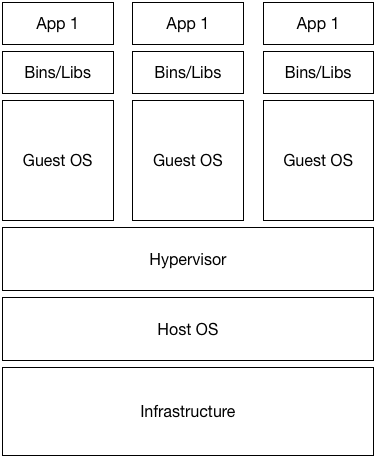
\includegraphics[width=0.4\textwidth]{tech/vm.png}
  \bicaption[fig:vm]{传统虚拟化技术示意图}{传统虚拟化技术示意图}{Fig}{}
\end{figure}

容器虚拟化技术并不是一个最近才出现的新技术,而是在2000年左右就已经有不少应用的虚拟化手段。

在容器虚拟化技术之前,比较常用的虚拟化工具有Xen,VMware等等。这些虚拟化工具都是属于Application Binary Interface级别的虚拟化,这样的虚拟化技术允许多个操作系统同时运行在同一套硬件上。这样的实现方式往往需要一个Virtual Machine Monitor,或者称作VMM的系统,来将硬件资源进行虚拟化,将虚拟机运行在虚拟化后的设备上。

而容器虚拟化技术是属于Application Programming Interface级别的虚拟化,每一个虚拟机,也被称为容器,只是操作系统上的一个进程,与普通的进程不同,容器使用namespace等等方式来将资源隔离,使得进程之间互相不感知。\cite{soltesz2007container}

相比于传统的虚拟化方式,容器虚拟化更加轻量,启动和销毁的速度快,资源消耗少。但与此同时,容器虚拟化也存在一些问题,首先是使用容器虚拟化的技术虚拟出来的容器,共用操作系统的内核。因此如果容器内导致了内核崩溃,那会影响到其他的容器。而使用Xen等技术,一个虚拟机的崩溃对于其他虚拟机而言,不会有任何影响。\cite{dua2014virtualization}

\subsection{Docker的核心概念}

Docker是目前被广泛接受的一种容器虚拟化工具,其有着其他容器虚拟化工具所不具备的一些优势。Docker原本是DotCloud公司的一个内部项目,DotCloud是一个专注于平台即服务的创业公司。在2013年3月13日,Docker发布了它的开源版本。它使用了内核中的lxc作为其容器的支持,同时还使用了内核中的cgroups和namespace的特性,因此需要内核支持。在Docker开源后,因为其便捷和高效的特性,受到了开发者的欢迎。在最初的版本中,Docker的网络等方面还不是特别的完善,但是Docker由DotCloud公司进行积极的开发和维护,在2014年的0.9版本中,Docker移除了lxc的依赖,直接与内核中的特性进行交互。并且亚马逊、IBM、微软Azure等等国际云服务提供商纷纷表示将整合Docker技术到其云计算产品中,一时之间Docker成为了云计算领域的热词。截止至2016年5月16日,Docker在Github上收获了31256个关注(Star),成为了Github上最受欢迎的项目之一。

\begin{figure}[!htp]
  \centering
  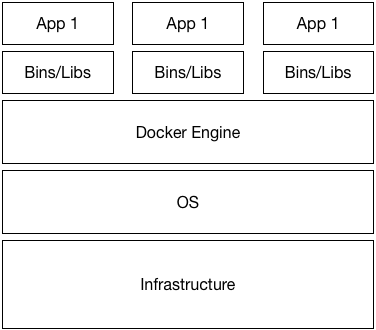
\includegraphics[width=0.4\textwidth]{tech/container.png}
  \bicaption[fig:container]{Docker示意图}{Docker示意图}{Fig}{}
\end{figure}

如图\ref{fig:container}所示,Docker不同于传统的虚拟化技术,每一个容器包含其运行时需要的所有依赖以及应用,但并不需要一个虚拟机来提供支持,每一个Docker容器只是一个运行在独立的namespace下的受到隔离的进程。与此同时,Docker容器不会跟下层的操作系统相耦合,它们可以运行在所有支持Docker Engine的机器或者云上。

Docker中比较重要的两个概念分别是镜像和容器,这是Docker最主要的两个实体概念。镜像是Docker的一个特色,镜像是一个只读的模板,在启动容器时被加载。镜像在存储方面,采取了联合文件系统。联合文件系统允许系统的文件和目录以分层的方式存储,而对于操作系统而言,其使用的文件系统是分层叠加之后的结果。这样使得镜像的存储变得更加方便,可以将不同的文件分层并行地进行上传或下载。而且当对镜像进行修改时,只需要对修改之后的文件分层进行添加或者修改即可,而不需要替换掉整个镜像。而Docker通过定义了一系列操作,将镜像的构建进行了标准化,使得用户只需要通过简单地操作,即可构建出满足自己需要的镜像。

而容器则是镜像的运行时,镜像为容器提供了启动的环境,而容器则与常规的容器虚拟化技术中的容器概念一致,是一个隔离的进程。因为Docker的镜像是一个只读的模板,其所有的文件分层都是设置为只读的,因此当从一个镜像运行起一个容器时,Docker会在镜像的最上层添加一个可读可写的新的文件分层。在新的文件分层中对于文件系统的修改,会覆盖原本的镜像。这样就使得容器看起来运行在镜像之上,而并不会因为容器的运行修改镜像的内容。

\subsection{Docker的架构}

\begin{figure}[!htp]
  \centering
  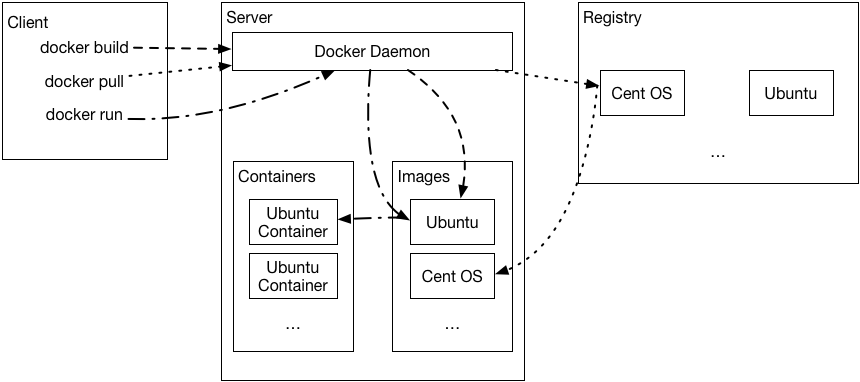
\includegraphics[width=\textwidth]{tech/architecture.png}
  \bicaption[fig:architecture]{Docker架构图}{Docker架构图}{Fig}{}
\end{figure}

如图\ref{fig:architecture}所示,Docker采取了客户端-服务器的架构。其中比较重要的组件有Docker Daemon,Docker Client,Docker Registry三个,下面将从镜像和容器的生命周期角度,对Docker的架构进行介绍。

Docker Daemon,是运行在服务器端的后台程序。其承担了基本所有的操作,包括本地镜像和容器的管理,与远端的Docker Registry的交互等等。但用户并不直接与Docker Daemon交互,而是通过Docker Client。Docker Client是一个Cli程序,为用户提供了抽象度很高的命令,通过Docker Client,用户可以与Docker的服务器进行交互,进而管理容器和镜像。而Docker Registry是管理镜像的存储组件,用户可以将构建好的镜像推送至Docker Registry中,而通过Docker Client,用户可以对Docker Registry上的镜像进行简单的搜索,寻找适合自己应用场景的镜像,并拉取使用。

\subsection{Docker的优势}

Docker有一系列优秀的特性。首先,作为一个容器虚拟化工具,它允许用户创建Docker容器,并且利用iptable等等特性,解决了容器与容器之间互相连接的问题。同时,Docker允许构建镜像,并且可以将镜像推送给远端的Registry,这使得一次构建,多次运行的想法成为了现实。而且Docker的Registry允许多租户,通过类似Github的方式来进行组织与构建,使得Docker在生产环境的使用成为了可能。

除此之外,Docker的成功也离不开其强大的生态环境。围绕着Docker,有一系列工具和技术覆盖了当下很多领域的难题。首先,Docker周边有非常多为了降低Docker的使用门槛的工具,比如Docker Machine等。原本因为容器虚拟化技术需要依赖Linux内核的某些特性,使得其他系统的用户不能使用Docker来构建容器,但是Docker Machine会在非Linux环境下运行一个Linux虚拟机,将Docker运行在该虚拟机上,这抹平了Docker对内核的要求,使得其他系统的用户也可以自如地使用Docker来构建容器,目前Docker正在积极基于OS X的新特性积极地进行对OS X系统的原生支持,这对于OS X系统的用户而言是一大利好。其次,Docker跨平台的特性,使得企业的混合云部署变成了现实。面对当下异构的机器和网络环境,Docker能够更好地发挥其特性。除此之外,在持续集成与持续部署方面,Docker非常用来做环境的隔离,执行构建任务。Drone等工具就是专注于该领域的,基于Docker来实现的工具。

%# -*- coding: utf-8-unix -*-
%%==================================================
%% impl.tex for SJTU Master Thesis
%%==================================================

%\bibliographystyle{sjtu2}%[此处用于每章都生产参考文献]
\chapter{系统需求分析与架构设计}
\label{chap:impl}

本章从需求角度和架构角度出发,介绍了Fornax在设计之初面临的功能性需求以及非功能性需求,并且基于这些需求,介绍了Fornax使用的架构,以及技术选型。

\section{需求分析}

持续集成与持续部署,已经成为了当下软件开发的最佳实践。因此也有越来越多的开发者希望能够在自己的开发流程中引入这样的实践来提高软件过程的效率与软件产品的质量。因此,持续集成与持续部署对于Fornax而言是非常重要的特性。持续集成要求Fornax必须与各种代码版本控制系统,比如Git,Svn等等进行交互。而持续部署要求Fornax要与应用的部署平台,也就是Kubernetes进行交互。

\begin{figure}[!htp]
  \centering
  \includegraphics[width=0.5\textwidth]{impl/vcs.png}
  \bicaption[fig:vcs]{代码与镜像的版本控制}{代码与镜像的版本控制}{Fig}{}
\end{figure}

而除此之外,Fornax作为基于容器集群的版本管理与发布系统,与其他的持续集成与持续部署工具比较大的不同在于,Fornax还需要负责对于软件应用构建情况的版本管理。在传统的软件过程中,只有代码是被纳入版本控制的,运行时的环境,依赖,都没有版本控制的概念。这样的实践存在一些问题,比如在代码被回滚时,往往需要同时将运行时环境,包括依赖一起进行回滚,而在传统的做法中,这样往往需要重新打包依赖,过程耗时长而且自动化程度低。在引入了容器后,情况产生了一些变化。容器技术引入的镜像,可以很好地解决对于依赖和环境的版本管理问题。每当用户代码被构建完成后,可以将整个运行环境,依赖,和代码打包成一个镜像,这样当需要回滚时,只需要根据之前已经打包好的镜像重新启动一个新的容器即可。这使得软件的开发与部署有了新的实践方式,而这也是Fornax希望实现的。如图\ref{fig:vcs}所示,Fornax希望能够将代码的版本管理结合Docker镜像的版本管理,在每次代码产生变动时,都构建一个Docker镜像,并将其推送到Docker Registry中,当用户遇到需要回滚代码时,不需要再重新检出代码之后再次进行构建,而是通过Kubernetes集群的Rolling back的特性,直接将容器回滚到前一个版本的镜像。这样使得持续部署和应用回滚成为了更加简单的特性。除此之外,对于用户的构建日志,需要进行持久化地处理,以便用户之后便于排查问题,这也是Fornax需要解决的问题。

上述是Fornax的功能性需求,除此之外,Fornax还需要满足一些非功能性的需求,比如需要保持扩展性较强的设计,来满足以后可能遇到的新的需求。以及保证自身的无状态性,便于在需要时对Fornax进行水平扩容,采取多实例的方式来保证Fornax能够比较便捷地进行分布式地部署,提高系统的可用性。

\section{系统工作流}

在Fornax中,有两个比较重要的概念,一个是服务,一个是版本。这两个概念模型贯穿了整个Fornax的生命周期。服务,是引申自微服务概念中的服务,是指一个代码仓库对应的概念。一个服务拥有自己的版本控制系统类型,以及仓库的地址等信息。而版本则相对于服务而言要更加复杂一些,版本是指一次构建的版本,其中包含构建的版本的名字,描述,以及该版本在集群上的部署情况,比如部署在哪个集群的哪个节点上的信息之类。在Fornax的设计中,一个版本对应一个Docker镜像,当用户需要回滚版本时,只需要对已经部署的容器进行镜像的回滚即可。服务和版本的概念串联起了Fornax的工作流。

在Fornax中,如果要使用其提供的基于容器集群的版本管理与发布服务,需要先建立一个与传统的版本控制工具,如Git,Svn等的仓库概念对应的服务,在建立服务后,相关于该仓库的信息就会被Fornax记录,之后每当代码发生了变动,都会由Fornax来进行一次版本的构建,版本的构建环节中,Fornax并不是简单地把代码打包成为一个Docker的镜像,而是一个相对于传统的版本管理与发布工具而言要复杂一些的步骤。

在Fornax的设计中,所有有关在构建时的配置等信息,是记录在一个YAML格式的配置文件中的。因此Fornax在收到一个构建版本的请求时,会先确定在Clone下来的仓库中是否存在这样的配置文件,如果存在,就会根据配置文件中的配置来执行相关的步骤,否则就会如同其他的工具一样,直接进行镜像的构建和发布。以下讨论都建立在仓库中存在该配置文件的基础上而进行。

\begin{figure}[!htp]
  \centering
  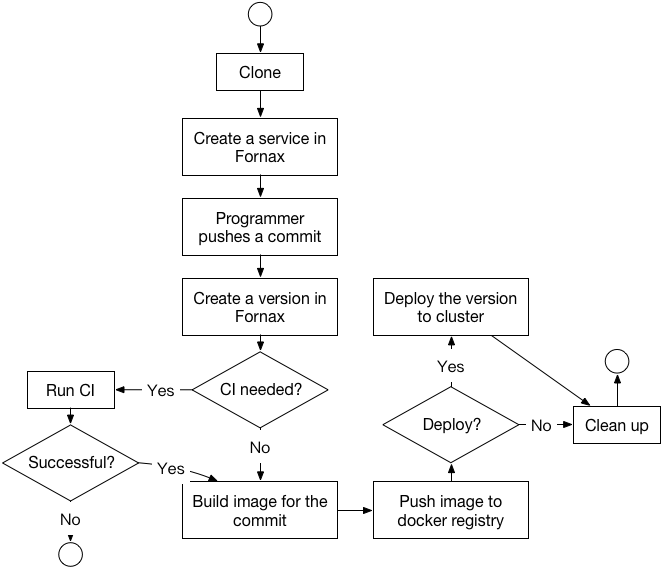
\includegraphics[width=0.7\textwidth]{impl/workflow.png}
  \bicaption[fig:workflow]{Fornax系统工作流}{Fornax系统工作流}{Fig}{}
\end{figure}

Fornax的工作流如图\ref{fig:workflow}所示,首先,Fornax会判断在配置文件中,是否有关于持续集成阶段的相关配置。如果存在这样的配置,Fornax会依据该配置文件,去进行相应的持续集成。通常持续集成的步骤会是执行持续集成测试,或者进行一些其他类型的测试以保证代码的质量,并根据持续集成的结果来判断是否需要打包新的版本。在Fornax中,持续集成的概念也是如此。在持续集成结束后,Fornax会根据结果来进行相应的操作,如果持续集成失败,那么整个流程都会结束,如果成功,Fornax会继续进行下一阶段的工作。值得一提的是,为了支持与现有的持续集成平台兼容,Fornax也允许使用Jenkins来进行持续集成,而不使用原本在Fornax中的持续集成,这样的妥协是为了保证能够尽快地接入现在主流的生产系统。

下一阶段的工作是构建和发布镜像。在这一阶段中,Fornax会在仓库中寻找目录下名为Dockerfile的文件,并根据该文件,去进行版本的构建。同时,为了满足一些自定义的需求,Fornax允许通过定义构建之前和之后的钩子(Hook)来执行一些用户定义的操作。在构建成镜像之后,Fornax会先将镜像存储在本地,在构建完成后,镜像会由Fornax推送到用户定义的Docker Registry或者推送到官方的Docker Registry上。

最后一阶段的工作是部署。在Fornax中,部署是指将打包好的镜像,在用户的集群中以容器的方式运行起来的过程,与持续集成相同,这也是自动化的过程。用户需要指定要部署的版本,选择集群,就可以将之前打包好的镜像发布到集群上。

在上述的阶段中,持续集成与持续部署是可选的阶段。而版本的构建会发布是每次代码发生变动时Fornax默认的行为。

\section{架构设计}

% 少了Daemon Manager

如图\ref{fig:design}所示,Fornax大致由八个模块构成。分别是API模块、异步事件管理模块、Docker管理模块、Docker后台管理模块、持续集成管理模块、版本管理系统管理模块、日志模块和数据库管理模块。这八个模块相互协同,实现了Fornax的所有功能。

\begin{figure}[!htp]
  \centering
  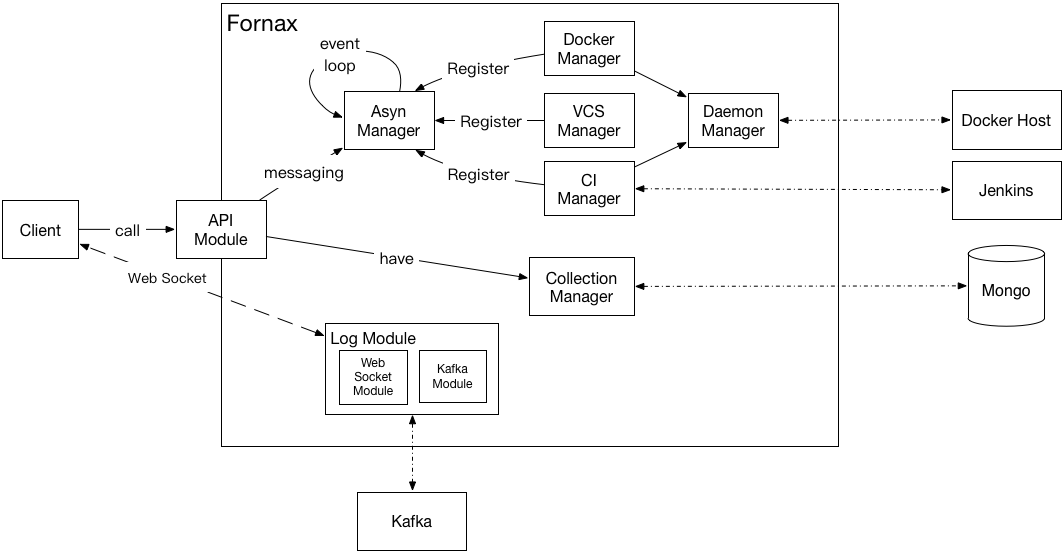
\includegraphics[width=0.9\textwidth]{impl/design.png}
  \bicaption[fig:design]{Fornax系统设计图}{Fornax系统设计图}{Fig}{}
\end{figure}

其中,API模块是将Fornax的服务以REST API的形式开放给客户端使用。这里的客户端不在Fornax的范畴内,可以是基于网页的客户端,或者是以命令行的方式来进行交互。API模块是整个Fornax系统对外交互的模块,它的职责在于接受来自客户端的请求,进行基本的认证与过滤,确保用户可信。之后,API模块会将过滤后的请求分发给相应的处理器进行处理。处理器也是API模块的一部分,他们会与异步事件管理模块交互,将请求交由其来进行调度与分配。

而异步事件管理模块,是其中比较重要的模块,也是实现难度比较大的模块。异步事件管理模块的职责是接受来自API模块发送过来的事件,然后将其加入到一个队列中,等待其被处理,并在处理后执行在API模块中定义的钩子函数,来进行自定义的收尾。异步事件管理器,是独立地运行在一个线程里的,不会阻塞主线程的运行,这也是异步操作带来的主要好处之一。目前Fornax中主要的两个事件是创建服务和创建版本,其他诸如查询服务内容,删除服务等等,因为处理起来比较快,不会过多地阻塞主线程,因此并没有进行异步化处理,而创建服务,涉及到对于代码仓库的Clone,创建版本,则不仅涉及该操作,还有持续集成任务的执行、镜像的构建、镜像的发布、容器的部署等一系列的事情,所以如果不以异步的方式去执行,会导致系统效率极低。因此Fornax对于这两种操作进行了异步的处理。

持续集成、版本管理、以及Docker构建镜像,都是在创建服务或者创建版本时需要使用的功能,所以三者对应的管理模块,会与异步事件管理模块交互,当一个事件在被处理时,异步事件管理模块会调用相应事件的处理器来进行处理,而三个模块就是在处理器中被其调用,进行相应的逻辑处理。

其中,版本管理系统管理模块负责与版本管理系统交互的功能实现。目前,版本管理系统管理模块包含Git,Svn对应的实现。当创建服务时,Fornax会将指定的代码仓库Clone下来,进行一些简单的校验。在创建版本时,为了防止代码仓库的污染,在每一步都会重新Clone代码仓库到Fornax指定的目录下。以及在发布镜像时,Fornax还会在发布的同时给构建镜像的提交打上一个标签,这同样需要版本管理系统管理模块支持。

Docker管理模块,是在构建和发布镜像时使用到的模块,Docker管理模块会与Docker Host进行交互,借由此来完成镜像的构建和发布。在目前的设计中,构建版本与服务时,对于Docker的依赖只限于构建镜像,和发布镜像,在持续集成环节中,还包括为每次持续集成构建隔离的网络环境等,这会在介绍持续集成管理模块时阐述。

Docker后台管理模块,是为了实现Fornax分布式的非功能性需求而实现的一个模块。在请求量比较大的时候,单个Docker Host必然没有办法满足Fornax的构建需要,因此引入了这样一个模块。该模块的职责是连接多个Docker Host进行构建,值得一提的是,该模块只有在定义了某些环境变量时才会被使用,默认情况下会使用一个Docker Host作为Docker的支持进行运行,这样设计是为了开发时的方便。

持续集成管理模块,是负责根据用户的仓库以及配置文件进行持续集成的模块。在Fornax中,持续集成是在容器内进行的。在一次持续集成中,Fornax会根据用户的配置,将用户自定义的持续集成以一个容器的方式运行起来。如果用户的代码存在运行时依赖,比如会依赖一个关系型数据库,Fornax也会支持通过容器方式先将用户在配置文件中定义好的依赖运行,再去运行用户自定义的持续集成的方式。依赖的容器和持续集成本身所在的容器通过自定义的网络环境相互连接,确保在一次持续集成任务中,容器间可以相互通信的同时,不会出现不同的持续集成任务之间容器可以相互沟通的问题,这是出于安全性的考量。持续集成管理模块,只有在存在配置文件,而且用户在配置文件中定义了相关持续集成阶段的配置时,才会被使用。

而日志模块,是相对独立的一个模块。它实现了一个基于WebSocket的协议,能够实时地将在各个阶段的日志推送给客户端。同时为了实现日志的持久化存储,引入了Kafka。具体实现的协议会在后文中进行更为详细的介绍。通过日志模块,用户可以在客户端看到每个阶段中所产生的日志。

最后,数据库模块,是对于数据库操作的封装。在API模块中,创建服务和版本都会向异步事件处理模块发送一个异步事件,而除此之外的所有操作,都只是单纯地通过对数据库的操作来完成。Fornax的数据库为MongoDB,是一个非关系型的数据库。因为服务与版本,都是非常灵活的模型。而为了满足这样的灵活性,非关系型数据库是比较好的选择,而MongoDB作为目前比较主流的生产可用的非关系型数据库,最终被采用。

上述八个模块,构成了Fornax。在第\ref{chap:detail}章中,会逐个介绍每个模块使用到的具体技术。

\chapter{Fornax实现细节分析}
\label{chap:detail}

本章从细节实现的角度出发,自顶而下地介绍了Fornax每个模块的具体实现。在第\ref{chap:impl}章中提到,API模块是Fornax与客户端交互的入口。因此对实现的具体细节分析,将从最顶层的API模块入手。

% 实现的细节分析
% 1. 持续集成(有service)
% 2. 构建与发布
% 3. 数据库设计
% 4. 日志消息

\section{Fornax初始化}

Fornax在实现上依赖很多外部的服务,其中包括MongoDB,Kafka,和Docker等。因此,如果要运行Fornax,必须有这些依赖的支持。为了实现依赖的可配置,Fornax采取了环境变量的方式定义这些依赖。表\ref{tab:env}列出了Fornax中所有的环境变量。其中前两项为MongoDB和Kafka服务所在的地址,通常是以IP或者域名的形式给出,而端口则是在两个服务启动时所在的默认端口。而DOCKER\_HOST和DOCKER\_HOST\_DIR是为了支持多个Docker Host做构建而定义的环境变量。而以REGISTRY为前缀的三个环境变量是与Docker Registry相关的配置,它们定义了地址与用户名密码,它们的作用会在之后进行更为详细的阐述。上面提到的环境变量是Fornax中为了解决依赖可配置而引入的,而其他的环境变量则是出于便于开发的目的,在此不做过多介绍。

在读取环境变量后,Fornax会将API模块中的所有API注册到一个HTTP服务器上,然后在主线程里运行该服务器,监听相应端口(默认为7099)。同时,Fornax会将额外启动一个线程来运行异步事件处理器的事件循环,事件循环可以被视为一个不会停止的循环,它接受一个通道(channel)的消息,并进行处理。还有一个WebSocket的服务器,同样会运行在一个独立的线程中,该线程主要负责将日志实时地推送给接收方。因此,在初始化后,Fornax会有三个线程在运行。

\begin{table}[!hpb]
  \centering
  \bicaption[tab:env]{指向一个表格的表目录索引}{Fornax环境变量配置}{Table}{}
  \begin{tabular}{ll} \toprule
    环境变量 & 描述 \\ \midrule
    MONGO\_DB\_IP & MongoDB服务地址 \\
    KAFKA\_SERVER\_IP & Kafka服务地址  \\
    DOCKER\_HOST & Docker Host地址  \\
    DOCKER\_HOST\_DIR & Docker Host目录 \\
    REGISTRY\_LOCATION & Docker Registry地址  \\
    REGISTRY\_USERNAME & Docker Registry用户名  \\
    REGISTRY\_PASSWORD & Docker Registry密码  \\
    DOCKER\_CERT\_PATH & Docker认证目录  \\
    ENABLE\_CAICLOUD\_AUTH & 是否开启用户认证  \\ \bottomrule
  \end{tabular}
\end{table}

\section{API模块实现}

% 有error?
\begin{table}[!hpb]
  \centering
  \bicaption[tab:api]{}{Fornax REST API}{Table}{}
  \begin{tabular}{lll} \toprule
    URL & 方法 & 描述 \\ \midrule
    /\{user\_id\}/services & POST & 创建新的服务 \\
    /\{user\_id\}/services & GET & 获得所有服务 \\
    /\{user\_id\}/services/\{service\_id\} & GET & 根据ServiceID查询服务 \\
    /\{user\_id\}/services/\{service\_id\} & DELETE & 根据ServiceID删除服务 \\
    /\{user\_id\}/services/\{code\_repository\}/requesttoken & GET & 根据用户请求私有仓库的Token \\
    /services/\{code\_repository\}/authcallback & GET & 授权的回调处理 \\
    /\{user\_id\}/services/\{code\_repository\}/listrepo & GET & 使用请求的Token列出所有仓库 \\
    /\{user\_id\}/services/\{code\_repository\}/logout & GET & 从Fornax中登出该Token \\
    /\{user\_id\}/versions & POST & 创建新的版本 \\
    /\{user\_id\}/versions/\{version\_id\} & GET & 根据ServiceID查询版本 \\
    /\{user\_id\}/versions/\{version\_id\}/logs & GET & 获得日志(默认无WebSocket支持)\\
    /\{user\_id\}/services/\{service\_id\}/versions & GET & 列出一个服务对应的所有版本 \\
    /apidocs & GET & API文档(默认不生成) \\ \bottomrule
  \end{tabular}
\end{table}

Fornax中的服务,是以REST API的形式暴露给外界的,而API模块就是对于REST API的封装。在之前的章节中提到,服务和版本是Fornax中两个最重要的实体概念。因此在REST API中这两个模型也是最主要的数据实体。Fornax所有的API在表\ref{tab:api}中列出。

% \begin{figure}[!htp]
%   \centering
%   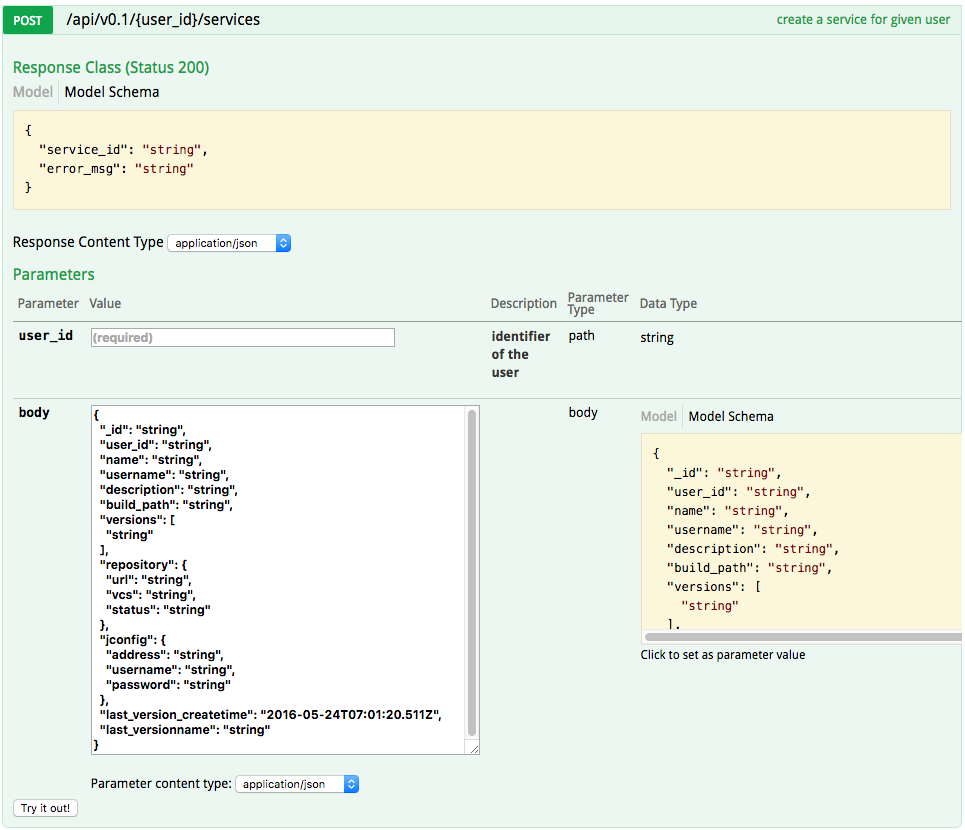
\includegraphics[width=0.9\textwidth]{detail/apidoc.png}
%   \bicaption[fig:api]{Fornax API文档图}{Fornax API文档图}{Fig}{}
% \end{figure}

通过定义了REST API,并将其与相应的逻辑处理器关联起来,最终以HTTP服务器的方式运行起来,以实现对外服务的功能。值得一提的是,Fornax在API模块中也实现了一项对开发者而言比较友好功能,即根据代码来直接生成REST API文档,而不再像是传统的方式那样,手动地维护一份API文档以供参考。在代码中定义REST API的部分,通过加入少量的说明,Fornax可以在运行时通过Flag的方式来决定是否将在运行的同时在/apidocs下生成一份API文档。首先,根据Fornax中原本的代码,会首先生成一个JSON格式的API规约,然后利用著名的API工具Swagger,产生一份人类可阅读的,HTML格式的文档。在API文档中不仅包括API的请求参数,以及返回的参数,还可以浏览到在代码中对应的相应的模型的定义,同时也可以直接通过文档发送请求,测试API的可用性。API模块的这一功能,使得外部与Fornax交互时可以感知到最新的接口,不会出现因为长时间没有维护API文档而导致的一系列问题。

\section{异步事件管理模块}

异步事件管理模块,是处理服务与版本创建的模块。在Fornax最初的设计中,所有的逻辑处理都是在主线程中完成,后来随着服务与版本在创建时的复杂性的提高,这样的设计不能满足需求,因此引入了异步事件管理模块,将创建服务与版本的过程异步化,使得它们不会阻塞主进程。异步事件管理模块的运行模型是传统的事件循环模型,异步事件管理模块的运行过程可以抽象为一个永远不会退出的循环,当收到来自API模块发送到来的消息时,会调用相关的处理器来处理该事件,并且会在处理结束后执行定义的钩子函数,来进行数据库操作,或者收尾工作等等。

\begin{lstlisting}[caption={抽象后的异步事件管理器结构与实现}]
type AsyncManager struct {
	operations map[Operation]OperationHandler
	events map[EventID]*Event
	newEvents chan *Event
	deleteEvents chan *Event
	lock sync.Mutex
}

func (am *AsyncManager) Start() {
	go func() {
		for {
			select {
			case event := <-am.newEvents:
				go func() {
					operationHandler, ok := am.operations[event.Operation]
					err := operationHandler(event)
					event.Lock.Lock()
					defer event.Lock.Unlock()
					// Deal with the error and call the post hook function.
				}()
			case event := <-am.deleteEvents:
				delete(am.events, event.EventID)
			}
		}
	}()
}
\end{lstlisting}

% \begin{algorithm}
% \caption{异步事件管理模块事件循环}
% \label{algo:eventloop}
% \begin{algorithmic}
% \LOOP
% \IF {there is a new event sent to the async event manager} 
% \STATE Create a new goroutine and call the handler function for the event.
% \ELSIF {There is a command to delete a event}
% \STATE Delete the event from the manager.
% \ENDIF 
% \ENDLOOP
% \end{algorithmic}
% \end{algorithm}

在其他语言中实现这样事件驱动的模型,是比较复杂的。而在go语言中,因为其对于通道(channel)和轻量级线程(goroutine)的支持,所以实现这样一个模型非常简单,这也是Fornax最终采取这样的模型进行异步化创建服务和版本任务的原因之一。异步事件管理器的数据结构如代码所示,其由一个以操作为键,以处理器函数为值的图、一个以事件的唯一标识符为键,以对应的事件的指针为值的图、以及两个通道和一个互斥锁构成。在执行Start函数时,首先会创建一个新的线程,并在该线程中进入一个无限循环,在循环中,会使用go语言中的select特性,来进行对事件的监听。如果接收到新的事件,就会去operations中寻找对应的处理器函数,并调用其进行处理。目前只有两种有意义的操作类型,即创建服务和创建版本,而因为两者之间不存在数据竞争,因此在进行处理时不需要加锁,只有在涉及到对事件本身的属性的修改时才需要加锁。

异步事件管理模块与Docker管理模块、持续集成管理模块、和版本控制系统管理模块在处理器函数中进行交互。在创建服务的过程中,Fornax会将用户指定的仓库Clone到本地,进行简单地校验,然后在结束时会将服务的元数据写入数据库。因此在创建服务的处理器函数中,会与版本控制系统管理模块进行交互。而在创建版本时,则会与三个模块都有交互。

\section{Docker管理模块}

Docker管理模块是在执行镜像的构建与打包时会被调用的模块。Docker管理模块会负责与Docker Host交互,当有创建版本的请求被发起时,会涉及到对于版本镜像的构建和发布。因此,Docker管理模块需要维护在构建与发布镜像时的所有信息。而且在构建镜像时,也需要对Docker Registry进行设定,保证用户可以从其可见的基础镜像中构建新的镜像。

\begin{lstlisting}[caption={Docker管理模块结构}]
type DockerManager struct {
  client     *docker_client.Client
  registry   string
  authConfig *AuthConfig
  endPoint   string
}
\end{lstlisting}

Docker管理模块的结构如代码所示,其中最主要的对象是Docker Client的抽象对象,该对象会负责与Docker Host进行交互,而诸如构建、发布等功能也是通过该对象进行的。而其他的对象,是在执行构建与发布时需要用到的参数。在构建与发布时,用户通常会将镜像推送到自建的Docker Registry上,这样的需求要求在进行构建与发布时,允许用户来指定一些用来认证的配置,以保证推送的成功。

\section{版本管理系统管理模块}

版本管理系统管理模块是唯一一个在创建服务与创建版本时都会使用的模块。不同于其他类型的模块,它们只有一种实现,版本管理系统管理模块因为需要适配多种版本管理系统,因此有着更高的抽象。

\begin{figure}[!htp]
  \centering
  \includegraphics[width=0.7\textwidth]{detail/vcs.png}
  \bicaption[fig:vcs]{Fornax版本管理系统管理模块UML类图}{Fornax版本管理系统管理模块UML类图}{Fig}{}
\end{figure}

由图\ref{fig:vcs}所示,版本管理系统管理模块向外暴露两个接口,分别对应着Clone操作和给一个指定的分支打上标签的操作。这两个操作会在异步事件管理模块处理相应事件时被调用。而为了满足适配多种版本管理系统的要求,版本管理系统管理模块将所有对于版本管理系统的操作抽象成了一个接口,由接口定义了一系列标准地,Fornax需要调用版本管理系统来支持的功能。而不同的版本管理系统需要分别实现对应的功能,以满足接口的要求。而对于版本管理系统的封装与版本管理系统管理模块是解耦合的,当需要使用其进行相应操作时,版本管理系统管理模块会根据用户的设定,先创建出操作对应的版本管理系统的对象,然后根据该对象进行操作。目前所有版本管理系统的实现是通过在go语言中调用Shell程序,来使用本地的版本管理系统的命令行工具来进行支持的。所以版本管理系统的封装本身是无状态的,因此重复创建并不会带来太大的开销。

一方面,go语言作为一门新兴的语言,目前没有能满足Fornax需求的对版本管理系统进行操作的第三方库支持,另一方面,调用Shell的方法可以满足现在的需求。所以Fornax采取了这样的方式来解决对于版本管理系统的依赖,在之后的愿景中,Fornax希望借助第三方库的支持,能够对版本管理系统进行更加准确地定义和使用。

\section{持续集成管理模块}

持续集成管理模块是Fornax中较为复杂的模块之一。其职责不仅包括对代码执行持续集成,还有对于除了构建与发布镜像之外的所有在创建版本时需要进行的操作,比如构建前的钩子,构建后的钩子,以及发布管理等等。因此这样的命名不能反应其明确的功能,但是在Fornax中还是以这样的方式去命名的,因为在最初时它只是为了进行持续集成而存在的。

\subsection{配置文件解析}

因为持续集成管理模块贯穿了创建版本流程的始终,因此对于该模块的实现介绍将从创建版本的流程出发。在创建版本的过程中,第一步是将仓库的代码进行Clone,接下来是解析代码中的配置文件。配置文件是用户定义的,与代码存放在相同目录下的一个YAML格式的文件。Fornax定义了一种语法与惯例,使得用户在按照语法将自己的需求以YAML文件的形式描述后Fornax可以根据该文件执行相应的操作。该文件默认名为caicloud.yml,如果在用户的仓库中存在以此命名的文件,Fornax会尝试解析该文件。这是持续集成管理模块的第一项职责。

\begin{lstlisting}[caption={配置文件格式}]
integration:
  image: <image name>
  environment:
    - <key>=<value>
    - <key>=<value>
  commands:
    - <cmd1>
    - <cmd2>
  services:
    <service name 1>:
      image: <image name>
      environment:
        - <key>=<value>
        - <key>=<value>
      commands:
        - <cmd1>
        - <cmd2>
    ...
pre_build:
  dockerfile_path: <path of the Dockerfile>
  image: <image name>
  environment:
    - <key>=<value>
    - <key>=<value>
  commands:
    - <cmd1>
    - <cmd2>
  outputs:
    - <path1>
    - <path2>
build:
  dockerfile_path: <path of the Dockerfile>
post_build:
  image: <image name>
  environment:
    - <key>=<value>
    - <key>=<value>
  commands:
    - <cmd1>
    - <cmd2>
deploy:
 - <application name>:
    cluster: <cluster name>
    partition: <partition name>
\end{lstlisting}

代码所示是一个完整的配置文件的规约。其中包括了五个阶段的配置信息,分别是持续集成、构建前、构建与发布、构建后、以及发布。在Fornax中,整个创建版本的过程都是由该配置文件进行控制的。用户可以通过定义各个阶段的配置,来确定构建阶段的行为。持续集成管理模块会对该配置文件进行解析,将其解析为一个运行时的树状结构,然后逐一执行。解析过程与传统编译器的词法分析器和语法分析器的实现类似,通过将配置文件的结构以结构体的形式定义,将配置文件解析为树状结构。树状结构可以直接被持续集成管理模块中的运行时所解释,从而根据配置执行相应的任务。

\subsection{执行树构建}

\begin{table}[!hpb]
  \centering
  \bicaption[tab:nodetype]{指向一个表格的表目录索引}{语法树节点类型}{Table}{}
  \begin{tabular}{ll} \toprule
    节点类型 & 描述 \\ \midrule
    NodeList & 根节点类型,用以构造多叉树 \\
    NodePreBuild & 构建前节点类型  \\
    NodeBuild & 持续集成中有关构建的节点类型  \\
    NodePostBuild & 构建后节点类型 \\
    NodeService & 持续集成中有关服务的节点类型  \\ \bottomrule
  \end{tabular}
\end{table}

执行树是一个多叉树结构,是由配置文件解析生成的,运行时执行的一个树状结构。表\ref{tab:nodetype}是树状结构中的节点类型。其中根节点是一个以节点为元素的列表。而其他节点类型都是以节点形式存在于该列表中。目前,执行树的深度最大为一,即所有的节点都直接与根节点相连。除了根节点外,其余所有节点都是一个包含了部分用户的配置信息的节点。而配置信息与节点的对应关系并不是一对一的,比如持续集成节点就对应着零个或多个服务节点,以及一个构建节点。因此执行树并不是一个语法树,而是一个由语法树得到的为了运行时而存在的结构。

运行时的环境除了执行树之外,还有一些用来进行资源隔离,以及与数据库等进行交互的对象。这些对象共同构成了持续集成管理模块的运行时环境。在运行时,除了根节点之外,所有的节点都与一个Docker容器对应。不同的阶段都对应着一个或者多个Docker容器,因此持续集成、构建前和构建后的钩子等等功能,都是通过Docker的容器机制实现的。

\begin{figure}[!htp]
  \centering
  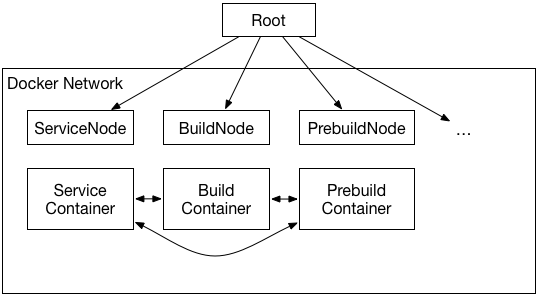
\includegraphics[width=0.7\textwidth]{detail/tree.png}
  \bicaption[fig:tree]{Fornax执行树模型}{Fornax执行树模型}{Fig}{}
\end{figure}

使用容器来执行各个阶段的任务,是出于资源隔离的考虑。容器本身具有轻量级,隔离性较好等特性,非常适合用来处理构建任务。构建任务需要在任务内所有的资源共享而构建任务之间应该具有良好地资源隔离性。为了实现这一要求,Fornax在网络,处理器,内存等的使用上都做了一些处理。首先从网络层面,为了保证构建内的所有容器可以相互交互而构建外的容器不可感知到其存在,Fornax使用了Docker的网络特性,为每一次构建都新建了一个Docker的网络。如图\ref{fig:tree}所示,在一次构建内,所有的容器都在一个为构建任务新建的Docker的网络中。在网络中,所有的容器都可以通过容器的名字或者定义的别名去对其他容器进行服务发现,这是由DNS的名字解析来实现的。而在同一个Docker Host中不允许有同名的容器,因此为了解决名字冲突问题,Fornax对需要暴露服务的容器会将其的名字以网络中的别名的形式出现,而对于容器名则进行一定的随机以保证不存在名字冲突。因此对于容器而言,其不感知自己名字而可以通过别名的方式让其他的容器与其进行交互。

引入Docker的网络是为了解决网络的隔离问题,而处理器和内存的隔离问题的解决相对而言要简单很多。容器本身在运行时就支持指定一定的处理器与内存配额,其实现方式取决于容器引擎的实现。目前Docker是依赖内核中的一些特性来实现的,其功能已经可以满足Fornax对隔离性的要求。因此Fornax会在启动容器时指定容器可用的最大处理器与内存配额,在之后Fornax的愿景是可以根据构建任务的需求,允许用户在一定的范围内指定配额,或者向用户推荐其最合适的配额。

除此之外,使用容器技术解决隔离问题,会涉及到代码目录应该如何映射到容器中的问题。因为对于一次构建而言,会有多个容器被启动。因此在容器中进行Clone是低效的选择,而Fornax使用Docker的数据卷特性,先把代码仓库Clone到本地,之后绑定到容器中,这样的实现方式也使得容器对于目录的修改会被保留在本地,在整个创建版本的流程中所有的工件都可以保留下来。

\subsection{持续集成}

持续集成是持续集成管理模块中比较重要,也是实现难度比较大的一个功能,对于持续集成的支持是Fornax在设计之初最重要的需求之一。对于用户代码的持续集成,不仅是允许用户对其代码执行一些简单的测试,也要同时支持在测试同时将用户的环境依赖运行起来,满足一些端到端测试的需要。因此,在持续集成中,也存在一个服务的概念。此处的服务与Fornax中的服务并不是同一概念,Fornax中的服务是与用户的仓库相对应的一个概念,代表了用户的一个功能模块。而在持续集成中的服务,是指用户的代码在运行时的环境依赖。比如一个典型的网站应用,会由前端、后端服务器和数据库组成,而对于前端的端到端的测试,需要将后端的服务器和数据库运行起来才能进行,而在持续集成的概念里,后端的服务器与数据库在此时即可被视为服务。而Fornax支持用户的持续集成对于服务的依赖,是使用容器技术来对其进行支持的。

在之前的配置文件一节中,配置持续集成不仅可以指定持续集成的命令,环境变量等,还有一个其他的阶段都不存在的配置,即服务配置。用户可以通过定义服务配置,在持续集成时先将服务运行起来,随后再执行定义的持续集成命令。因此在持续集成阶段,会有多个容器被启动,容器之间都会被加入到同一个Docker的网络中以相互通信。在持续集成结束后,Fornax会先将所有的容器都删除,之后再将构建中使用的Docker的网络删除,保证没有构建垃圾的残余。如果持续集成完成,会继续执行树结构上的其他节点,完成创建版本的流程,而如持续集成失败,就会返回错误,结束所有流程。因为对于构建垃圾的清理,以及数据库操作等都是以异步事件管理模块中的钩子来实现的,所以无论成功与否,都不会留下残留的垃圾,这也是异步事件管理模块在设计上的一种好处。

在持续集成时,持续集成管理模块会与Docker管理模块共用一个Docker Client对象,因此目前Docker管理模块与持续集成管理模块会有所耦合。

\subsection{构建时钩子}

Fornax支持构建前和构建后的钩子,由于两者所运行的时间不同,因此有不同的实现。对于构建前的钩子而言,往往是为了配合构建。在有关Docker的生产实践中,两个Dockerfile完成构建的应用场景越来越多,而这样的应用场景只通过构建与发布的过程,并不能得到满足。而引入了构建前的钩子,就可以满足这样的需求。在实现上,Fornax会在持续集成结束后,再次根据构建前的钩子运行一个容器,该容器会执行在配置中定义的内容,而且采取了绑定目录的方式解决目录问题,所以在构建前的钩子中所产生的输出在构建时刻都是可见的。

构建后的钩子是为了执行一些用户定义的发布任务。因为在一些应用场景中,用户不仅仅需要产出一个版本镜像,还会有一些自定义的内容需要发布,构建后的钩子就是来解决这样的需求的。相比于其他的步骤而言,其实现较为简单,以一个容器的方式运行,并且执行用户定义的脚本。

\subsection{部署}

除了构建与发布之外,所有的环节都由配置文件所控制。因此在部署时,也是由用户在配置文件中写明要部署的具体集群与位置,Fornax会负责与其后的容器集群进行交互,完成部署任务。在部署时,是通过集群的REST API与其进行交互。因此相对于容器集群而言,Fornax是一个服务的前端,用户可以通过原本的方式进行部署,也可以在Fornax中使用配置的方式完成自动部署。

\section{Docker后台管理模块}

Docker后台管理模块是为了更好地解决并发构建而引入的模块。通过Docker网络的支持,Fornax使得每次构建之间不会出现端口的冲突,而这并不能完全解决并发的构建问题。除此之外,还存在一个问题,就是在同一时间内的同一个镜像,Docker只允许有一个镜像被推送,而这样是不能满足Fornax的需求的,因此需要引入Docker后台管理模块来解决该问题。

Docker后台管理模块是在开发的后期被引入的一个模块,它会管理多个连接不同Docker Host的Docker管理模块,可以被理解为是维护一个可用的Docker管理模块的资源池的模块。当需要使用Docker管理模块进行镜像的构建与发布时,Fornax会向Docker后台管理模块请求一个空闲的Docker管理模块实例,之后的操作中会使用该实例进行镜像的推送与发布。

\section{日志模块}

日志对于Fornax而言的重要性毋庸置疑。而Fornax为了保证日志可以准确而实时地推送给用户前端的同时,保持Fornax的资源高效利用,因此设计了一套基于WebSocket的与客户端进行通信的简易协议。该协议允许Fornax与客户端建立WebSocket连接,在有日志产生时,实时地将日志推送给用户端。同时在用户端一定时间内没有回应时,Fornax会自行关闭该连接,以保证不会因为保持过多的连接造成资源的浪费。

日志模块的实现依赖Kafka,一个使用阿帕奇许可证开源的高吞吐量的分布式消息中间件系统。Kafka支持发布者-订阅者的模式,对一个指定的主题(Topic)进行订阅,订阅者会在有新消息被提交时收到该消息。Fornax会在每次构建时,新建一个Kafka的主题,该主题会对应一次构建,在该构建中的所有日志都会发送至该主题。而Fornax会负责将主题持久化,并且在有订阅者订阅该主题时进行推送。

在Fornax中,通过Kafka实现了对日志的订阅,而与客户端进行交互则是使用了WebSocket连接。WebSocket是在RFC 6455\supercite{websocket}中被提出来的一种建立在单个TCP连接上的全双工的通信协议。它允许服务端向用户端主动地推送数据或信息,这正是日志推送所需要的功能。

\begin{figure}[!htp]
  \centering
  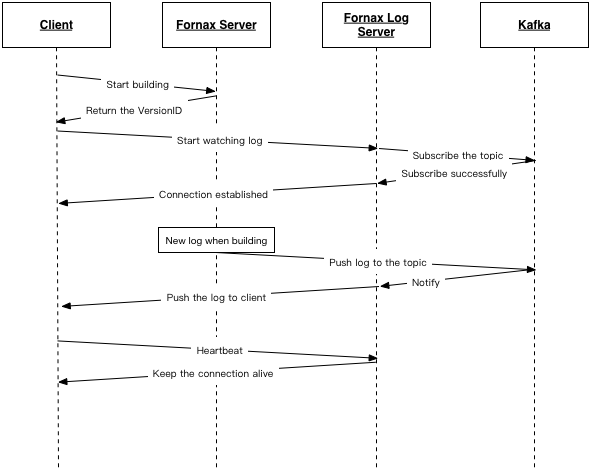
\includegraphics[width=0.9\textwidth]{detail/log.png}
  \bicaption[fig:log]{Fornax日志模块交互图}{Fornax日志模块交互图}{Fig}{}
\end{figure}

为了实现日志实时推送的功能,Fornax在其主线程之外还有一个监听其他端口的日志服务器线程,该服务器只负责有关日志获取的部分逻辑。它从Kafka中获取日志,并将其推送给订阅相关日志的客户端。客户端、Fornax主服务器线程、Fornax日志服务器线程与Kafka之间的交互如图\ref{log}所示,当客户端发起一次构建时,Fornax会先生成一个唯一的标识符代表这次构建产生的版本,而随后会由异步事件管理模块调度构建的运行。在运行时,构建产生的日志会由Fornax推送给Kafka,而指定的主题是由发起构建的用户唯一标识符,构建所在的服务的唯一标识符,和代表该次构建的唯一标识符拼接而成。所有在构建时的日志都会被推送至该主题中。

因此,所有构建时的日志都会推送至Kafka中,而Fornax日志服务器线程,其本质是一个只与Kafka进行交互的独立线程。它会监听一个独立于Fornax主线程的端口,接受来自客户端的请求并处理。当接收到来自客户端的请求时,Fornax日志模块会去订阅相应的日志主题,然后当Fornax在构建时的日志被推送到Kafka中时,日志管理模块就可以订阅到该推送,并借由之前建立的连接推送至客户端,完成日志的推送工作。

为了完成这一步,Fornax设计了一个简单的应用层通信协议,保证日志可以实时准确地推送到客户端的同时不会占用过多的资源。首先,客户端会与Fornax的日志管理模块建立WebSocket连接,以便客户端与Fornax之间进行通信,客户端与Fornax通信的数据格式为JSON。请求与返回的数据包格式如表\ref{tab:protocol-client}和表\ref{tab:protocol-server}所示。在客户端想订阅日志时,会先向Fornax发送一个数据包,该数据包有如表\ref{tab:protocol-client}所示的字段。其中第一个字段动作在客户端发往Fornax的请求中会被置为查看日志,而接口字段会被统一置为创建服务或者创建版本,因为只有在创建服务或者版本时Fornax才有日志被写入Kafka中。而后面的用户、服务、与版本的唯一标识符是为了确定请求对应的具体日志。此时是客户端向Fornax发送的第一个包,用以通知Fornax该客户端希望订阅一个具体的日志。因此请求包中的日志字段为空,操作字段会被置为开始,以通知Fornax该客户端希望开始接收该次构建的日志推送。而唯一标识符则是唯一的标识该包的字段,会被设为一个自动生成的通用唯一识别码(Universally Unique Identifier)。通用唯一识别码的目的在于唯一的标识该包,在客户端与Fornax密集通信时保持请求与回应的一致。

\begin{table}[!hpb]
  \centering
  \bicaption[tab:protocol-client]{指向一个表格的表目录索引}{Fornax日志模块请求的数据包格式}{Table}{}
  \begin{tabular}{ll} \toprule
    字段 & 说明 \\ \midrule
    action & 动作 \\
    api & 接口 \\
    user\_id & 用户名 \\
    service\_id & 服务唯一标识符 \\
    version\_id & 版本唯一标识符 \\
    log & 日志内容 \\
    operation & 操作 \\
    id & 唯一标识符 \\ \bottomrule
  \end{tabular}
\end{table}

\begin{table}[!hpb]
  \centering
  \bicaption[tab:protocol-server]{指向一个表格的表目录索引}{Fornax日志模块返回的数据包格式}{Table}{}
  \begin{tabular}{ll} \toprule
    字段 & 说明 \\ \midrule
    action & 动作 \\
    reponse & 返回 \\
    id\_ack & 请求的唯一标识符 \\
    error\_code & 错误码 \\
    error\_msg & 错误信息 \\ \bottomrule
  \end{tabular}
\end{table}

在Fornax收到动作字段为查看日志的请求包,并且该包中操作字段为开始时,会返回一个包以表示收到该请求包,返回的包格式如表\ref{protocol-server}所示,在返回的包中,动作字段统一会被置为返回,而返回字段会被置为收到请求,请求的唯一标识符字段会被置为之前请求包中自动生成的通用唯一识别码,而错误码为零,错误信息会置为成功。与此同时,日志模块会创建一个新的线程,并且在线程中创建一个Kafka的消费者对象,该对象会订阅根据请求中用户、服务、版本三个唯一标识符而确定的唯一的日志主题,随后会向与客户端建立的会话中推送包含日志信息的数据包。这是由Fornax主动推送给客户端的包,其格式与客户端向Fornax发起的请求包格式一致,但字段的值会有所不同。其动作字段会被置为推送日志,而不是查看日志。而接口字段仍然与客户端的请求包中保持一致,其后的用户、服务、版本三个唯一标识符也同样与客户端的请求包中保持一致。而相比于客户端向Fornax发送的请求包,两者最大的不同在于其日志字段不再为空,而是会根据Kafka中订阅的主题获得的日志数据来进行发送。客户端在接收到Fornax发送的日志推送包时,会返回一个格式如表\ref{tab:protocol-server}所示的包,以通知Fornax该包已经被接收。

在Fornax中,日志模块是运行在一个单独的线程中的。在日志写入Kafka的部分实现中,是使用了本地与Kafka相互配合的方式来进行的。首先,关于构建的日志会写入到一个临时文件中,这是最开始Fornax的实现。而在开发中发现将日志信息存储在本地不利于Fornax的分布式部署,因此在之后的实现中引入了Kafka的依赖。在引入Kafka后,Fornax同样会先将日志信息存储在本地的文件中,而在每次构建时,会启动一个新的线程去监听日志文件的变化。目前监听的实现方式是轮询,每隔一定的时间间隔Fornax会重新访问本地的临时日志文件,将变动以消息的方式发送给Kafka。日志写入Kafka的实现是日志模块与Fornax主要功能想耦合的一部分,在进行构建时会调用该部分实现进行日志的写入。

而将日志发送给客户端是独立于Fornax主要功能的实现,是一个单独的服务器线程。在该部分实现中,日志模块会启动一个监听端口的服务器,并维护一个活跃的WebSocket连接的会话列表。该服务器只提供一个接口,即建立客户端与日志模块的连接。在连接建立后,日志模块会直接通过连接与客户端进行交互。日志模块在交互时定义了两个通信的接口,分别是查看日志与发送心跳。客户端可以对日志模块发送这两种类型的请求包,其中查看日志是前文中提到的由客户端第一次发给Fornax日志模块的请求包,而心跳是为了维持连接而由客户端定时地发送给Fornax日志模块的请求包,心跳请求会更新对应会话的最后活跃时间。

从实现来看,日志模块是一个相对独立于Fornax的模块,在后续对分布式部署实现的分析时会说明这样设计的目的。

\section{数据库管理模块}

数据库管理模块,是Fornax与MongoDB进行交互的操作对象。在实现上,一共由两个管理器构成,即服务管理器与版本管理器。在Fornax被启动时,在初始化时会创建两个管理器的全局实例,随后会在API模块以及异步事件管理模块等模块中被使用。该模块的实现较为简单,是一层对于MongoDB中Collection的操作的封装。使得Fornax可以在代码中直接操作MongoDB中的对象。

% 如图\ref{}所示,在Fornax的数据库设计中,一共有两个Collection,分别是服务与版本。
%# -*- coding: utf-8-unix -*-
%%==================================================
%% test.tex for SJTU Master Thesis
%%==================================================

%\bibliographystyle{sjtu2}%[此处用于每章都生产参考文献]
\chapter{验证与测试}
\label{chap:test}

本章从功能验证和测试的角度阐述了Fornax的功能与性能。并且通过对于同类型产品的比较,对Fornax的特点进行了说明。

\section{功能性测试}

作为着眼于持续集成、持续发布以及版本管理的系统,Fornax对于代码的质量有严格的保证,其具有完善的测试用例,并使用Jenkins作为持续集成工具,对于每次提交进行持续集成测试,在确保不会引入问题时才会将代码合并。目前Fornax在运行时会依赖数据库组件MongoDB和消息中间件Kafka,而Kafka作为开源的消息中间件实现,本身还会依赖分布式协调一致组件Zookeeper。因此,如果要进行端到端测试,需要先将这三个服务运行,Fornax才能被正确地启动。

\begin{figure}[!htp]
  \centering
  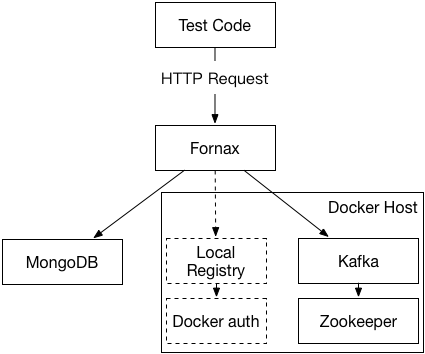
\includegraphics[width=0.55\textwidth]{test/test.png}
  \bicaption[fig:test]{Fornax测试架构图}{Fornax测试架构图}{Fig}{}
\end{figure}

如图\ref{fig:test},Fornax会将Kafka和Zookeeper以Docker容器的方式启动,将数据库启动在本地,除此之外,为了测试版本的推送功能,Fornax需要一个Docker Registry进行验证,而测试的应用场景对于Docker Registry有着不同于平时的需求,其要求Docker Registry的生命周期足够短,在测试结束时不能留下残余垃圾。因此使用公共的或者私有的Docker Registry都不能满足这样的要求,因此在Fornax启动之前,一个私有的Docker Registry会被启动,随之而存在的用以认证的一个服务也会随之启动。这两个服务也是以Docker容器的方式运行的。随后Fornax会被真正地运行,而测试代码是独立于Fornax实例而存在,其本质是模拟Fornax的客户端,对Fornax发起HTTP请求以测试Fornax在行为级别的表现是否满足预期,而针对Fornax的代码,有一些异常路径的测试用例被执行,因此属于端到端的测试,也可以被视为灰盒测试。

目前,Fornax中具有35个端到端的测试用例,覆盖了Fornax的全部的主要流程和部分异常流程。Fornax使用行为驱动的测试风格维护这些测试用例,使得在新增用例时代码不会过于膨胀。在35个测试用例中,有11个用例测试有关服务的逻辑,15个用例测试有关版本中构建与发布的逻辑,还有额外的9个用例专门关于给定配置文件后构建版本时的逻辑。因为在创建版本时版本镜像的构建与发布是默认的行为,因此相比于给定配置文件后进行构建的应用场景要更常见一些,所以书写了更多的测试用例。但从代码复杂度而言,给定配置文件后进行构建要比直接构建与发布镜像要复杂许多,因此在之后Fornax会补充更多完善的关于根据配置文件进行构建的测试用例。

\section{分布式部署}

Fornax作为一个生产环境可用的版本管理与发布的工具,支持分布式的部署方式。Fornax本身是无状态的,因此在分布式的支持上有很多种选择,而Fornax目前采取的方法是使用了第三方的反向代理工具,对Fornax进行请求的代理。Fornax进行分布式部署的目的在于提高系统的可用性以及请求的吞吐量,使得Fornax能够真正成为一个生产环境可用的工具。

\begin{figure}[!htp]
  \centering
  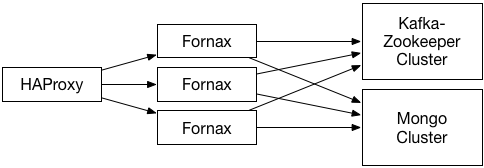
\includegraphics[width=0.55\textwidth]{test/distributed.png}
  \bicaption[fig:distributed]{Fornax分布式部署}{Fornax分布式部署}{Fig}{}
\end{figure}

如图\ref{fig:distributed}所示,Fornax在分布式部署中使用到了HAProxy作为反向代理的工具。在结构上主要分为Fornax集群,Kafka集群和Mongo集群。Fornax集群中每个实例的关系是完全对等的,都是无状态的。而Mongo集群和Kafka集群是使用其默认的分布式部署的支持方式进行部署的,它们为多个Fornax的实例提供服务。每当有请求路由到HAProxy时,HAProxy会根据自身的负载均衡策略将请求分发至一个具体的Fornax实例,该实例收到由其路由过来的请求后,会对其进行处理,并将服务,版本等信息存储到数据库集群中,而有关日志的信息会存储到消息中间件集群中。

在最开始的设计中,Fornax对于日志的处理上是使用本地文件,而不是消息中间件的方式来实现的。这样的实现方式在将Fornax进行分布式部署的尝试时遇到了问题。使用本地文件来存储日志信息使得Fornax本身不是完全无状态的,这要求对于同一个构建,其相关的请求都要路由到同一个Fornax实例上,因为对于构建的日志是存储在实例所在机器的本地的,而这样的分布式部署并不能真正起到提高可用性的目的。因此在后期的实现中Fornax引入了Kafka的依赖,讲日志也持久化在分布式的消息中间件中,所有的Fornax实例都连接该分布式的消息中间件,因此无论客户端请求在哪个Fornax实例上进行构建任务的日志,任意一个Fornax实例都可以订阅Kafka中的主题,来将日志推送给客户端。这样的实现是的Fornax成为了无状态的服务器,所有需要持久化的数据都下沉到了数据库与消息中间件中。而因为Fornax是无状态的,而且所有的实例都使用同一个数据库集群和消息中间件集群,所以连续的请求不需要路由到同一个实例上,这也是Fornax可以采取这样的分布式架构的主要原因。因为Fornax是无服务的,所以在部署时,Fornax实例是以Docker容器的方式运行的。而反向代理工具HAProxy也是以这样的方式进行部署,这使得Fornax的弹性扩容能力与可用性都相比于传统的部署方式有很大的提高,可以面对未来复杂多变的应用环境。

与此同时,Fornax的可配置性好,允许对所有的依赖进行配置,使得依赖由静态变成了动态的过程。同时Docker容器化的部署使得Fornax不感知真实的环境,因此无论是在公有云、私有云亦或是混合云,Fornax都可以进行部署。

% \section{性能测试}

\section{代码统计}

Fornax代码情况使用cloc\cite{cloc}统计,去除了Fornax中对于其他模块的代码依赖。情况如表\ref{tab:code}所示,Fornax的主要功能由go语言实现,其中包括八个核心的模块,以及所有的测试用例,因此go语言的代码占代码总量的大部分。除此之外,Fornax在启动时有很多的运行时依赖,这些依赖的运行以及Fornax的启动都是通过Bourne Shell脚本来完成的,其中包括启动本地的短生命周期的Docker Registry,启动Fornax,执行端到端的测试等内容。

\begin{table}[!hpb]
  \centering
  \bicaption[tab:code]{指向一个表格的表目录索引}{Fornax代码统计}{Table}{}
  \begin{tabular}{lllll} \toprule
    语言 & 文件数 & 注释 & 代码 \\ \midrule
    Go & 62 & 1129 & 6671 \\
    Bourne Shell & 15 & 96 & 375 \\
    YAML & 11 & 4 & 249 \\
    HTML & 1 & 0 & 31 \\
    make & 1 & 8 & 12 \\
    总计 & 90 & 1237 & 7338 \\ \bottomrule
  \end{tabular}
\end{table}

\section{相较于其他工具的优势}

Fornax关注持续集成与持续部署,版本的管理与发布,是两者的结合。在业界,有不少与Fornax具有类似功能的工具,比如Jenkins、Drone、Travis CI等。而这些工具跟Fonnax之间存在着一些功能的差异,以及思想的不同。本节将从这些工具的差别的角度出发介绍Fornax的优势。

Jenkins,Drone,Travis CI都是关注持续集成的工具。它们在实现上各有不同。Jenkins是三个工具当中最早,也是最流行的持续集成工具。其实现并没有借助容器虚拟化的技术,而只是通过操作系统的进程,目录等等进行了简单的隔离。不过Jenkins支持主从结构的分布式部署,经历过真实使用的考验。Jenkins采用Java实现,代码简洁易懂,插件众多,扩展性好。同时,Jenkins提供了网页和API两种方式进行构建,API使用XML格式作为传输格式。因此在配置的可读性上,比以YAML格式的配置文件难以阅读。但这并不影响Jenkins是目前市场份额最大的开源持续集成工具。在Fornax的实现过程中,也是使用Jenkins来对Fornax进行持续集成,保证Fornax的代码质量的。

Drone是一个新兴的持续集成工具,与Fornax一样,是使用go语言实现的,其在持续集成过程的工作流与Fornax类似,都是采取了YAML格式的配置文件来控制整个持续集成流程的方法。Drone本身的目的是取代Jenkins成为持续集成工具的下一代主流,因此就功能而言与Jenkins相差无几。而从实现角度而言,Drone与Fornax相同,使用了Docker来进行构建时的隔离,其同样支持插件,并且有命令行工具支持,可以通过命令行直接与Drone进行交互,完成构建,对于开发者而言更加友好。相比于Jenkins,Drone使用了更多的新技术与新工具,使得代码实现更加简洁的同时,拥有更好地隔离性。Drone也支持分布式的部署,它允许接入多个Docker Host来进行分布式的构建。

Travis CI是另外一款开源的持续集成工具,主要使用Ruby语言实现。Travis CI的功能与前两者并无区别,只是另一种的实现思路。Travis CI对于隔离的方式有更多的选择,并且其在日志传输等方面更加成熟。在其开源的版本中,有使用容器来进行构建隔离的实现。

\begin{table}[!hpb]
  \centering
  \bicaption[tab:advantage]{指向一个表格的表目录索引}{Fornax与其他工具对比}{Table}{}
  \begin{tabular}{llllll} \toprule
     & 实现语言 & 持续集成 & 分布式 & 容器隔离 & 版本管理 \\ \midrule
    Jenkins & Java & 支持 & 支持 & 不支持 & 不支持 \\
    Drone & Golang & 支持 & 支持 & 支持 & 不支持 \\
    Travis CI & Ruby & 支持 & 支持 & 支持 & 不支持 \\
    Fornax & Golang & 支持 & 支持 & 支持 & 支持 \\ \bottomrule
  \end{tabular}
\end{table}

Fornax与其他工具的对比如表\ref{tab:advantage}所示,Fornax也如其他工具一样,具有持续集成的功能,并且使用了容器虚拟化技术对构建进行隔离,保证构建之间互相不感知。Fornax可以通过HAProxy来进行分布式的部署,以满足更高的吞吐量要求。而Fornax不仅是一个专注于持续集成的工具,同样是一个版本管理与发布的平台。对于其他的持续集成工具,每次构建只会留下日志。而对于Fornax而言,不仅日志会保留,每次构建在成功时还会构建并且发布一个版本镜像,这也是Fornax与其他的持续集成工具最大不同所在。而且Fornax在解决发布的问题上与其他的工具也存在不同。Fornax目前是一个专用性的工具,只关注将应用部署到Kubernetes集群上。这意味着Fornax可以根据这样的应用场景做适配与优化。

因此,Fornax在定位上与现有的持续集成工具存在一定的差异,持续集成不是Fornax唯一的功能,相比于其他的持续集成工具,Fornax更加关注对于版本的管理,以及将应用部署到容器集群上的过程。这也是Fornax的优势所在。
%# -*- coding: utf-8-unix -*-
%%==================================================
%% conclusion.tex for SJTUThesis
%% Encoding: UTF-8
%%==================================================

\chapter{总结与展望}

本部分总结了Fornax目前已经完成的工作,并对Fornax的未来进行了展望。

\section{工作总结}

本文基于容器技术和容器集群技术,实现了一个用于版本管理与发布的系统,名为Fornax。通过Fornax,用户可以对自己的代码进行持续集成,并且在持续集成结束后,将代码打包成容器镜像的格式,上传至远端的仓库。在部署时,可以通过Fornax的持续部署,根据新打包的镜像直接在指定的集群上运行容器。同时,Fornax允许用户在构建镜像时定义自己的操作,使得可以在打包镜像的同时时完成用户定义的逻辑。

并且Fornax在实现时使用了容器虚拟化技术来进行构建任务之间的隔离。一次构建任务由一个或多个容器完成,容器间通过网络互连,而不同构建任务之间的容器之间互相不感知。同时Fornax是一个异步的、无状态的服务,因此通过第三方的负载均衡器的代理,可以实现分布式部署,提高Fornax的吞吐量以及可用性。

在最后,课题针对Fornax的功能进行了端到端的测试,测试覆盖了Fornax的全部正常工作流与一些异常流。通过测试的方式来验证Fornax的功能符合规约,同时证明功能实现的完整性。

\section{未来的工作}

Fornax的代码托管在Github上,而在Github的问题页面,已经积累了大大小小四十多个有关Fornax的问题,其中有优化,也有因为Bug而导致的问题。由此可见目前Fornax还不是非常完善,有很多工作需要未来一点点去完成。下面将从几个需要关注的方面着手,展望Fornax未来需要解决的问题。

首先是关于日志模块,在日志推送时,因为最开始使用了本地存储的方式,所以在后续引入Kafka来将日志推送至分布式消息中间件的实现中仍然有本地存储的依赖。目前每多一个构建请求,都要创建一个线程去监听本地日志文件的变化,然后将其推送给Kafka。后续应该调研是否仍然有必要使用本地存储,是否可以直接将日志推送至Kafka消息中间件中。这样可以节省很多的处理器资源。

其次是关于持续集成模块,在目前,虽然持续集成已经可以进行,但是还存在一些问题。比如,在构建失败时,有可能因为路径问题而没有回收构建时产生的垃圾。另外,目前对于用户所使用的硬件资源并没有作出限制。当用户在一次构建中创建出过多容器占用了整个机器的硬件资源时,会影响其他构建任务的执行。而为了解决这一问题,需要比较大的改造。对于用户占用资源的控制,可以分为三个维度,分别是对容器的资源限制,对构建任务的资源限制,和对用户的资源限制。对容器的资源限制是指要限定每个容器可以使用的硬件资源,这由内核的特性提供支持。内核中的cgroup和namespace特性使得这不需要Fornax实现。而对于构建任务的资源限制是指在一次构建中所启动的所有容器使用的硬件资源的总和应该进行限制。对于用户的资源限制,是指用户的多次构建任务所占用的硬件资源的总和也应该予以限制。三个维度的资源限制都是有必要的,而目前Fornax只能做到第一个维度的限制。对于第二个维度的限制,需要Fornax维护构建任务中所有容器的信息,并实时地进行计算。而对于第三个维度的限制,则相对比较困难,需要将用户的构建信息写入数据库,来进行判断。

类似这样的问题还有诸如在一次请求中数据库访问次数过多,以及用户校验以及鉴权等等。这些问题都是未来Fornax需要解决的问题。

\appendix	% 使用英文字母对附录编号,重新定义附录中的公式、图图表编号样式
\renewcommand\theequation{\Alph{chapter}--\arabic{equation}}	
\renewcommand\thefigure{\Alph{chapter}--\arabic{figure}}
\renewcommand\thetable{\Alph{chapter}--\arabic{table}}
\renewcommand\thealgorithm{\Alph{chapter}--\arabic{algorithm}}

%% 附录内容,本科学位论文可以用翻译的文献替代。
% \include{tex/app_setup}
% \include{tex/app_eq}
% \include{tex/app_cjk}
% \include{tex/app_log}

\backmatter	% 文后无编号部分 

%% 参考资料
% \phantomsection
% \addcontentsline{toc}{chapter}{参考文献}
\bibliography{bib/thesis.bib}

%% 致谢、发表论文、申请专利、参与项目、简历
%% 用于盲审的论文需隐去致谢、发表论文、申请专利、参与的项目
\makeatletter

%%
% "研究生学位论文送盲审印刷格式的统一要求"
% http://www.gs.sjtu.edu.cn/inform/3/2015/20151120_123928_738.htm

% 盲审删去删去致谢页
\ifsjtu@review\relax\else
  %# -*- coding: utf-8-unix -*-
\begin{thanks}

在本科学位论文的写作过程中,受到了很多老师、同学以及其他的朋友们的帮助。

首先,最需要感谢的是我的导师任锐老师。从项目的立项,到后来的实现,再到最后的论文写作,任老师都给予了很多中肯的意见,使得我在实现系统,撰写论文时绕过了很多弯路。同时任老师对待工作与学术的认真也给我留下了极深的印象。

其次,还需要感谢才云科技的邓德源、高建桥和陈曦先生。才云科技是一家容器集群即服务的创业公司,在Fornax的实现过程中提供了很多帮助。在实现过程中经常与邓德源先生进行深入的讨论与交流,受其指导颇多,收获也很大。

与此同时,还要感谢实验室里同一级的同学们,包括张坚鑫同学、孙浩然同学以及李彤宇同学。我们为了毕业设计一起努力,之后的三年时间里希望能够与三位同学继续保持这样的态度读过在交大的研究生生活。

最后,要感谢我的父母,他们给了我很大的自由空间,让我可以按照自己的心意读过大学四年的生活。他们也是我最坚强的后盾,愿他们健康。

除此之外还有很多值得感谢的人,在这里不一一列举了,希望能够在以后能再次与各位合作交流,也谢谢大家一直以来的帮助,使我能够顺利完成学位论文的写作。

\end{thanks}
 	  %% 致谢
\fi

\ifsjtu@bachelor
  % 学士学位论文要求在最后有一个英文大摘要,单独编页码
  \pagestyle{biglast}
  %# -*- coding: utf-8-unix -*-
\begin{bigabstract}
Operating-system-level virtualization has been the hottest topic in Computer System and Cloud Computing. Docker is the most popular implementation of operating-system-level virtualization, it allows the programmers to build, ship and run their applications easily. Docker is hosted on Github, with 31256 stars by Mar 16th, 2016. Since Docker is now generally acceptable, there are many services and tools based on it. Kubernetes is a open-source system for automating deployment, operations, and scaling of containerized applications. The ecosystem of Docker is growing up rapidly.

Fornax is a release management system, which is built on Docker. Fornax aims to provide the continuous integration, continuous deployment and version control of microservices. 

Continuous integration is a main feature in Fornax. Every time the programmers push their local changes to the remote repository, which is taken over by a specific version control system, such as Git or SVN, Fornax would create a continous integration task and run the customized commands. And Fornax is designed to integrate with popular CI tool like jenkins, to facilitate existing infrastructure. 

Continuous deployment is an important software engineering approach to agile software development. Fornax integrates with Kubernetes, to deploy microservices. When the integration test passed, Fornax would build a conatiner image from the commit, push it to registry, and deploy it to the container cluster. And Fornax allows to declare which cluster and which partition to deploy, and support to deploy on multiple cloud architectures such as public cloud, private cloud or hybrid cloud. The deployment cloud be flexible.

Those two features make the Fornax a available continuous integration or continuous deployment tool, and the support for version control of microservices makes Fornax meet the demand of the modern software process. Repository in the traditional version control system is equivalent to a service in Fornax. Fornax would take over the version control of the programmers' application. So Fornax integrates with version control systems and Docker image service to make both code and runtime of the applications traceable and able to roll back.

There are two concept in Fornax, service and version. Service is equivalent to a repository in the version control system. And version contains the code by a commit and a Docker image built from the code. A service would have more than one version, and the version could deploy to Kubernetes cluster. Fornax has a reasonable workflow, First The programmers should input the necessary information, including the URL of repository, the type of verson control system and the token for authorization if needed. Fornax would create a service for the repository, and check whether the information is correct. When the service is created successfully, Fornax would take over the version control of the service. When a commit is pushed to remote repository, Fornax would start a continuous integration task. If the task passes, Fornax would build a Docker image from the code, push it to the customized Docker Registry and store the information of the version. If the programmers have defined the settings about continuous deployment, Fornax would deploy the new version to user-defined cluster. From the perspective of programmers, they just need to push their commit to remote, and Fornax will take over the continuous intergation, version control and continuous deployment.

Fornax has eight components: API module, async event manager, Docker manager, version control system manager(VCS manager), continuous integration manager(CI manager), Docker Daemon manager, log module, and datebase collection manager. 

API module wraps the Fornax as REST API. Fornax run as a HTTP server, listening a specific port. All the requests would reach the API module first and API module would filter the requests, ensure the requests are valid, then would handle the requests. It's a lot of time to create services or versions, so it is asynchronous. When API module receives the requests to create services or versions, it would send a event to async event manager.

Async event manager schedules the event queue, it receives the events sent from API module, and handle these events asynchronously. There are two kinds of events: create services and create versions. Async event manager uses channels, the feature in golang, to perform a event loop. And it will integrates with Docker manager, CI manager and VCS manager to deal with the two kinds of events.

Docker manager is a wrapper around Docker Client. Fornax would build and push the image to Docker Registry by Docker manager. And To push the image isolatedly, Fornax implements Docker Daemon manager to manages multiple Docker manager. When async event manager should call Docker manager to push the image, it would acquire a idle Docker manager from Docker Daemon manger, then push the image to Docker Registry.

VCS manager is a wrapper around the version control systems, Continuous integration requires some VCS operations, so Fornax need to import the VCS bundle. Now VCS manager supports Git and SVN, and in the future, other version control systems would be adapted.

CI manager is the most important module in Fornax. CI manager take over the life cycle of a version, from continuous integration and deployment. First, CI manager would check whether the file named caicloud.yml exists. The file is the config during creating version process. It defines the operations that should be executed when the version is created. If the file doesn't exists, the CI manager wouldn't work, and Fornax just builds and pushes docker image to Docker Registry. Then CI manager parses the config file, and run continuous integration, before-build-hook, build, push, post-build-hook and deploy one by one. 

At the continuous integration step, CI manager would run the dependencies and the service as containers, these containers would communicate with each other via DNS name resolution. CI manager promises that the containers in one request would discover each other, but containers in different requests could do that. 

At the before-build-hook and post-build-hook step, CI manager would run a single container, and execute the customized commands. Fornax supports the hooks to improve usability.

Build and push are two default steps in Fornax. A version could have some optional steps to run, such as continuous integration or before-build-hook, and two default steps, build and push. In these two steps, Fornax would build the docker image, and push it to Docker Registry.

CI manager is a monolithic module, and in the future, CI manager would be refactored.

log module is another module, which is focuing on logs during the version creating process. At first, Fornax stores logs locally. With the increase of throughput, Fornax shuold be deployed as a distributed application. So log module imports Kafka, an open source messaging system, to store logs in the distributed architecture. And log module communicates with the clients by WebSocket, WebSocket allows Fornax to push real-time logs to client.

Datebase collection manager wraps the connection to MongoDB, Fornax would store the services and versions into MongoDB by database collection manager. It's a global module exposed to all other modules.

To avoid serious bugs, Fornax has many sound test cases. There are 11 test cases about services and 24 test cases about versions. The test cases are end-to-end, and covers the main workflow of Fornax and some alternative flow. These test cases help us keep the code in high quality.

And with the growth of throughput, Fornax imports HAProxy, an open source load balancer to distribute. Fornax is designed to stateless, so the requests could route to an arbitrary Fornax instance. Distributed architecture improves the availability, makes Fornax production-ready.

Although Fornax is production-ready, it also has a lot of problems to solve, especially in CI manager and log module. In some situation, CI manager could recycle the containers and the network, which would cause the resource leak. And log module now is not stable enough, in the future, Fornax would fix these problems to make it much more robust.
\end{bigabstract}

\else
  % 盲审论文中,发表学术论文及参与科研情况等仅以第几作者注明即可,不要出现作者或他人姓名
  \ifsjtu@review\relax
    \include{tex/pubreview}
    \include{tex/projectsreview}  
  \else
    \include{tex/pub}	      %% 发表论文
    \include{tex/projects}  %% 参与的项目
  \fi
\fi

% \include{tex/patents}	  %% 申请专利
% \include{tex/resume}	  %% 个人简历
% \makeatother

\end{document}
